
\documentclass[12pt,a4paper,oneside]{article}
\usepackage[margin=1.2in]{geometry}
\usepackage{appendix}
\usepackage[dvips]{graphicx}
\usepackage{epsfig}
\usepackage{amsmath}
\usepackage{amssymb}
\usepackage{psfrag}
\usepackage[square, comma,sort,numbers]{natbib}
\usepackage{fancyhdr}
\usepackage[nottoc]{tocbibind}
\usepackage{color}
\usepackage{fixltx2e}
\usepackage{pdfpages}
\usepackage{pdflscape}
\usepackage{booktabs}
\usepackage{graphicx}
\usepackage{float}
\usepackage{afterpage}
\usepackage{subcaption}
\usepackage{lscape}
\usepackage{rotating}
\usepackage{enumitem}
\usepackage{array,tabularx}
\usepackage{fancyref}
%\usepackage[dvipsnames]{xcolor}
\usepackage[colorlinks=true,allcolors=blue]{hyperref}%
\usepackage[table,xcdraw]{xcolor}


\newcommand{\quotes}[1]{``#1''}

\newenvironment{conditions*}
  {\par\vspace{\abovedisplayskip}\noindent
   \tabularx{\columnwidth}{>{$}l<{$} @{\ : } >{\raggedright\arraybackslash}X}}
  {\endtabularx\par\vspace{\belowdisplayskip}}



\pagestyle{fancy}
\title{\Huge The Hat Creek Radio Observatory\\
\vspace{0.5cm}
GReX Electromagnetic Interference Measurements\\
\vspace{0.5cm}
\normalsize \emph{}
\vspace{3.5cm}
\begin{center}

\includegraphics[height=4cm]{Figures/SETI_institute_logo.jpg}
\end{center}
}
\author{ 
\vspace{1cm}
\Large
\textbf{Alexander Pollak, Wael Farah, Marc Jacquart} \\
SETI Institute \\ 
339 Bernardo Ave, Suite 200 \\
Mountain View, CA 94043 \\ 
Alexander.Pollak.87@gmail.com\\
}
\date{\today}



\begin{document}
\clearpage\maketitle
\thispagestyle{empty}

\newpage

%----------------------------------------------------------------------------------------
%	General
%----------------------------------------------------------------------------------------

This document summarizes the testing of the GReX electronics' EM interferences at the Hat Creek Radio Observatory (HCRO) on April 3rd, 2024.

\section{Measurement setup}
\label{sec:Testing}

The GReX unit is place in the HCRO's screened room and it's electromagnetic emissions are recorded by a spectrum analyzer connected to an omnidirectional antenna through a signal amplifier. A schematic of the setup is shown in figure \ref{fig:measurement_setup_schematics}, a list of the components used in table \ref{tab:setup_component_list} and a picture of the setup inside the screened room is shown in figure \ref{fig:screened_room_setup}. A list of settings for the spectrum analyzer is shown in table \ref{tab:spectrum_analyzer_settings}. One modification was done for all the tests, compared to the state in which the GReX module was received: steel wool was added in the opening for the fiber cable to further shield the GReX enclosure.

A first baseline measurement was done with all the GReX electronics turned off. Then, the GReX was powered on and the emission spectrum was recorded for the GReX enclosure closed and opened separately. The SNAP board was programmed with the ``2023-08-16\_1325'' firmware after switching the unit on, but the 10 Gigabit Ethernet output was not enabled. As a final test, RF absorbers were placed in the GReX enclosure and the emission spectrum was once again measured with the enclosure closed. The hypothesis tested here is that the GReX enclosure acts as a resonant chamber for the EMI. Adding absorbers in the enclosure would reduce the interferences inside the enclosure, thus reducing the amount escaping the enclosure causing interferences on the outside.

\begin{figure}[H]
\centering
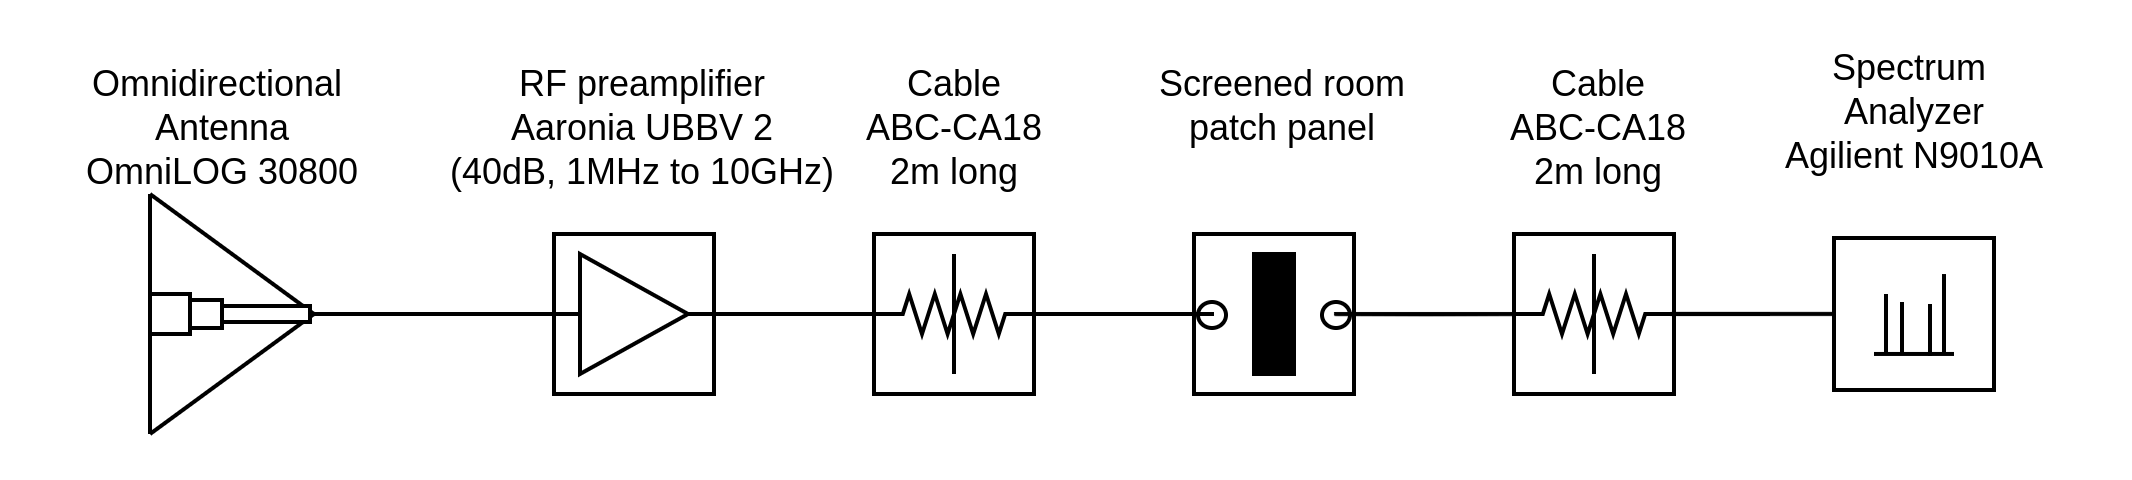
\includegraphics[width=1\linewidth]{Figures/measurement_setup_schematics.png}
\caption{GReX EMI measurement setup schematics.}
\label{fig:measurement_setup_schematics}
\end{figure}
%
\begin{figure}[H]
\centering
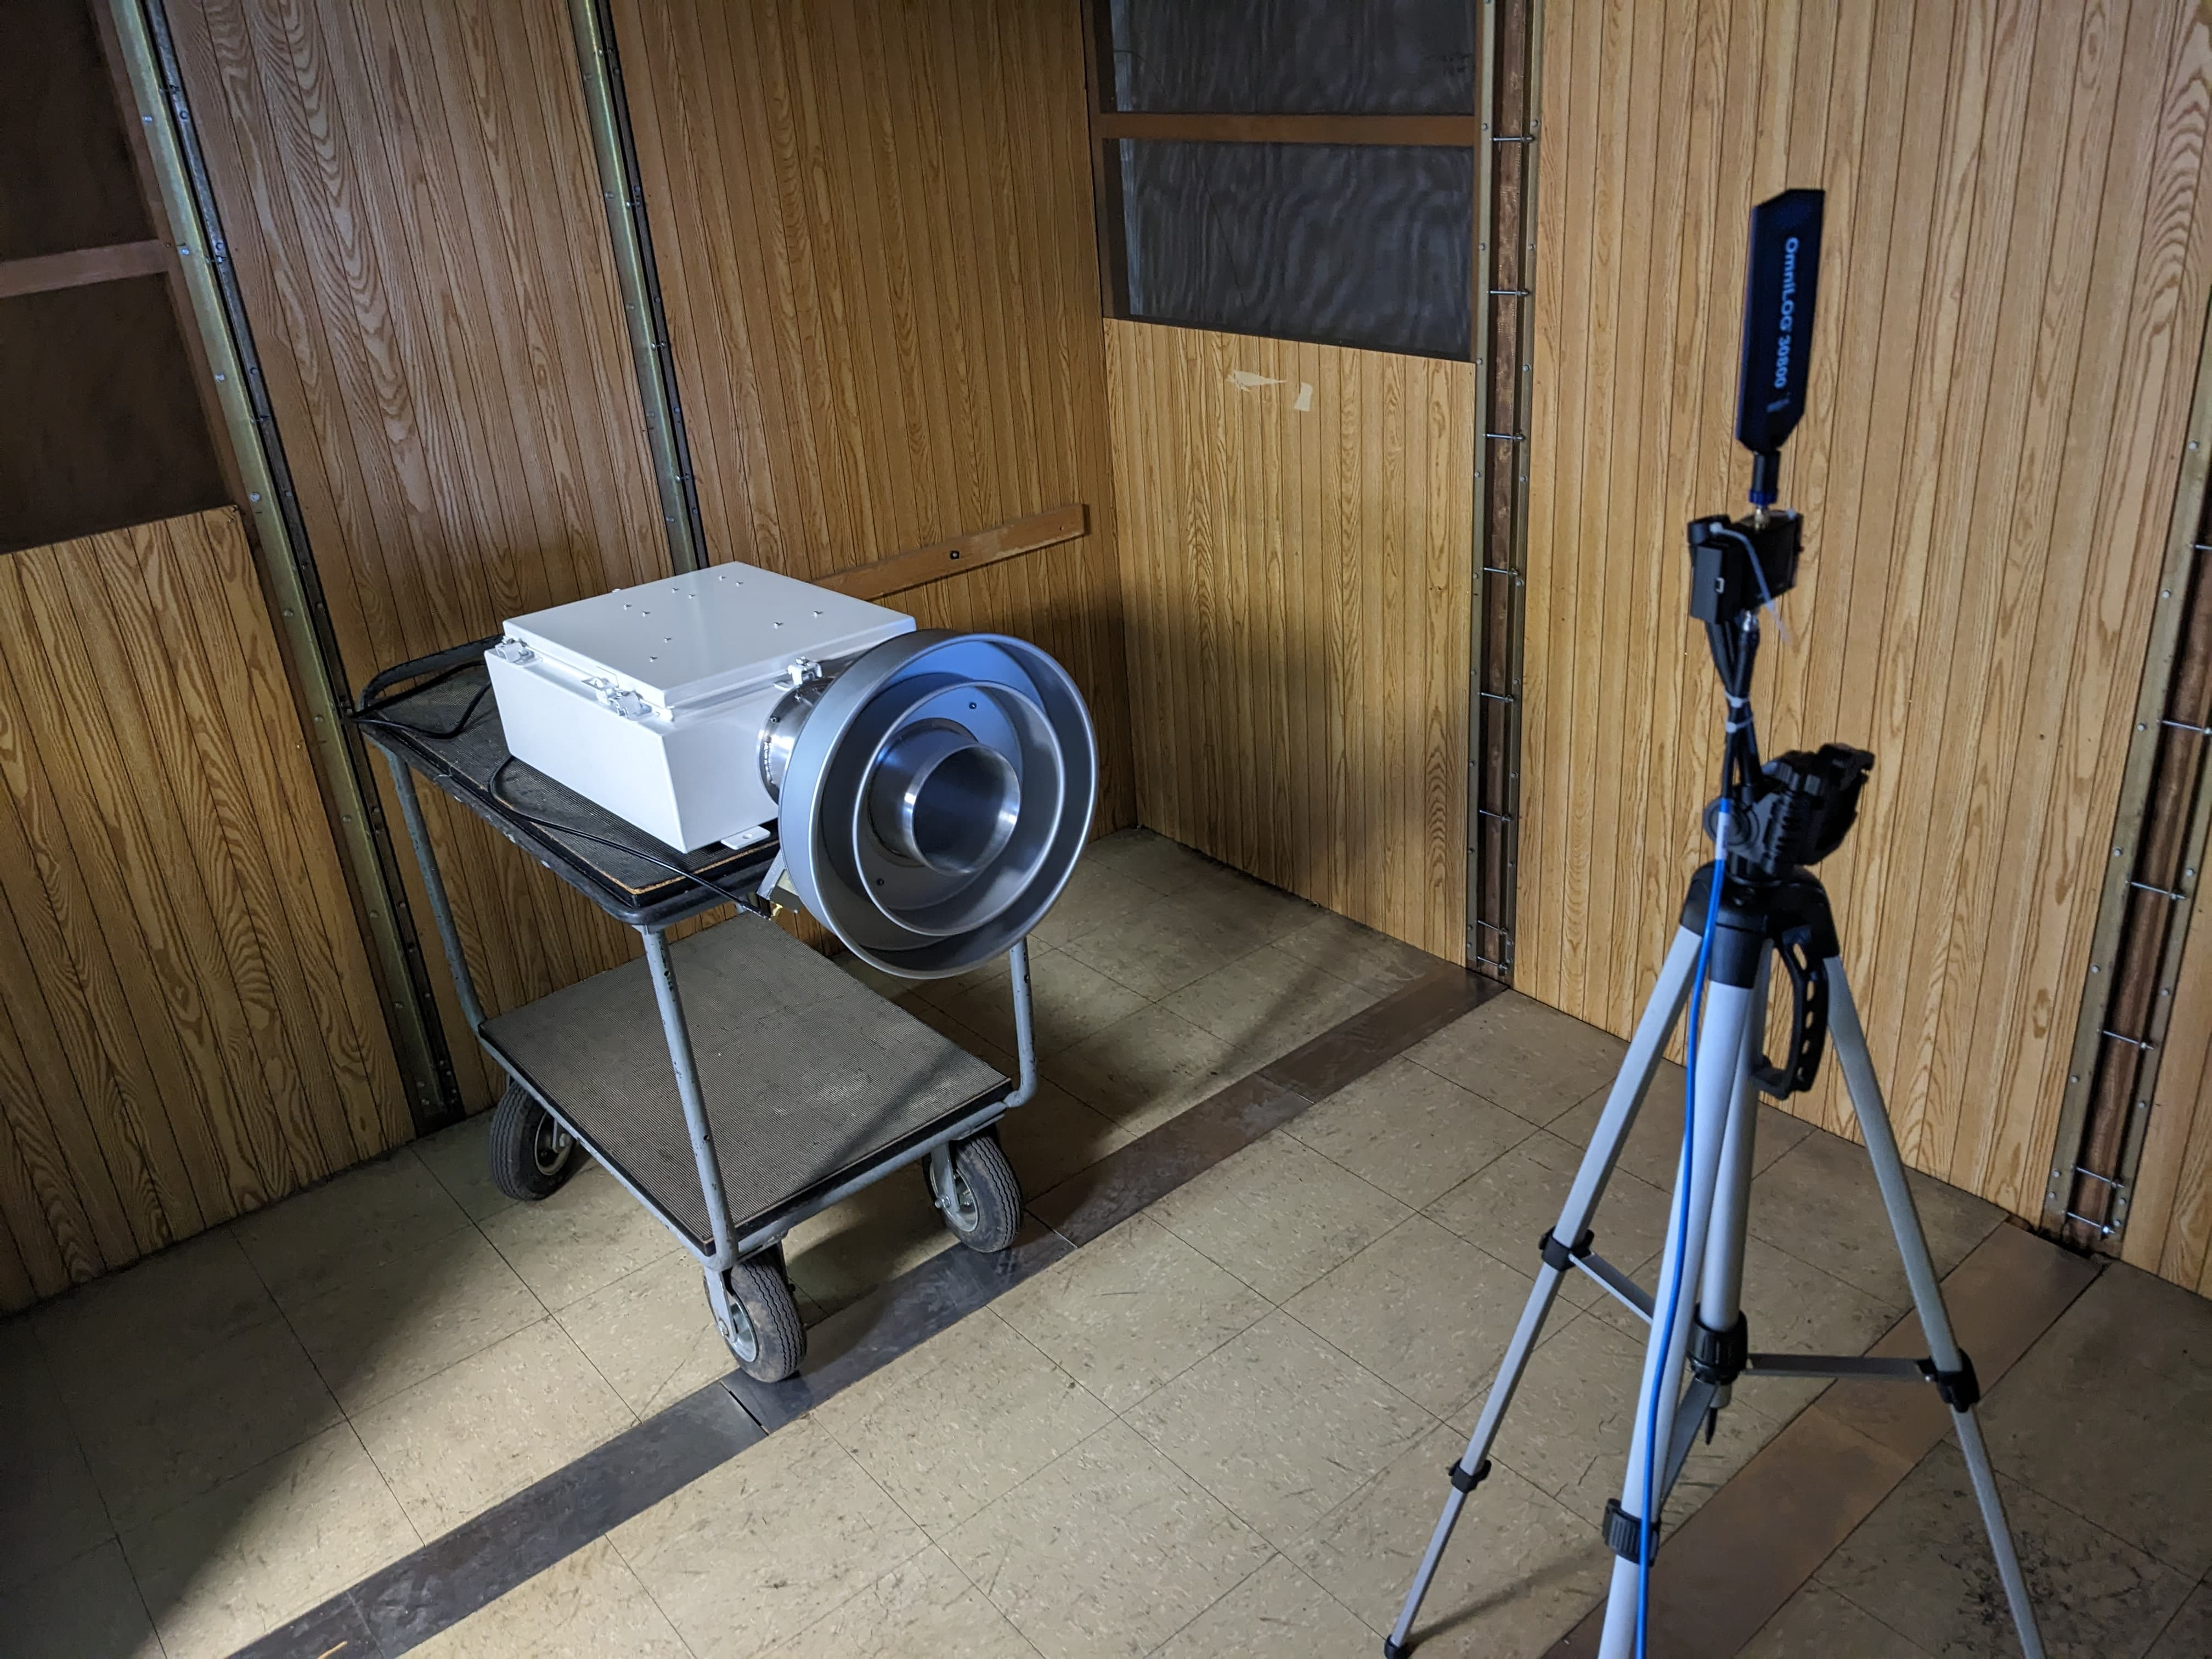
\includegraphics[width=0.8\linewidth]{Figures/screened_room_setup.jpeg}
\caption{GReX EMI measurement setup in the HCRO screened room.}
\label{fig:screened_room_setup}
\end{figure}
%
\begin{table}[]
    \centering
   
    \begin{tabular}{|c|c|}
    \hline
         \cellcolor[gray]{0.85} Description & \cellcolor[gray]{0.85} Designation \\ \hline
         Omnidirectional antenna & OmniLOG 30800\\ \hline
         RF preamplifier & Aaronia UBBV 2\\ \hline
         Female-Female SMA cable 2m & ABC-CA18-SMSM-2.OM\\ \hline
         Female-Female SMA cable 5m & ABC-CA18-SMSM-5.OM\\ \hline
         Spectrum analyzer & Agilent N9010A\\ \hline
    \end{tabular}
    \caption{Components list for the GReX EMI measurements.}
    \label{tab:setup_component_list}
\end{table}

\begin{table}[]
    \centering
   
    \begin{tabular}{|c|c|}
    \hline
         \cellcolor[gray]{0.85} Description & \cellcolor[gray]{0.85} Setting \\ \hline
          Start Frequency & $300\thinspace$MHz \\ \hline
          Stop Frequency & $6\thinspace$GHz \\ \hline
          Number of points & 1001 \\ \hline
          Sweep time & 656.176 s\\ \hline
          RBW & $100\thinspace$Hz \\ \hline
          VBW & $1000\thinspace$Hz \\ \hline
          Attenuation & 0 dB\\ \hline
          Trace type & Maxhold \\ \hline
          Detector & Peak \\ \hline         
    \end{tabular}
    \caption{ Agilent N9010A specrum analyzer settings list for the GReX EMI measurements.}
    \label{tab:spectrum_analyzer_settings}
\end{table}
% ----------------------------------------------------------------
\section{Results}
\label{sec:Results}

The baseline spectrum is shown in figure \ref{fig:baseline_result}. The emission peaks around $1\thinspace$GHz are due to the EMI emitted by the spectrum analyzer itself, even though it is set outside the screened room for the measurements. However, this contribution is negligible compared to the GReX measurements shown below. Figure \ref{fig:open_result} shows the spectrum for the GReX enclosure open. The spectrum measurement result with the GReX enclosure closed is shown in figure \ref{fig:closed_result}. Finally, figure \ref{fig:absorber_comparison_spectrum} shows the effect of adding absorbers inside the enclosure. These four spectra are respectively referred below as ``baseline'', ``open'', ``closed'' and ``absorber''. A list of the highest interference peaks, defined as a value greater than $30\thinspace$dB above its neighbors and a distance of at least 5 spectrum values between each peaks, is reported in table \ref{tab:main_emission_peaks}.

\begin{figure}[H]
\centering
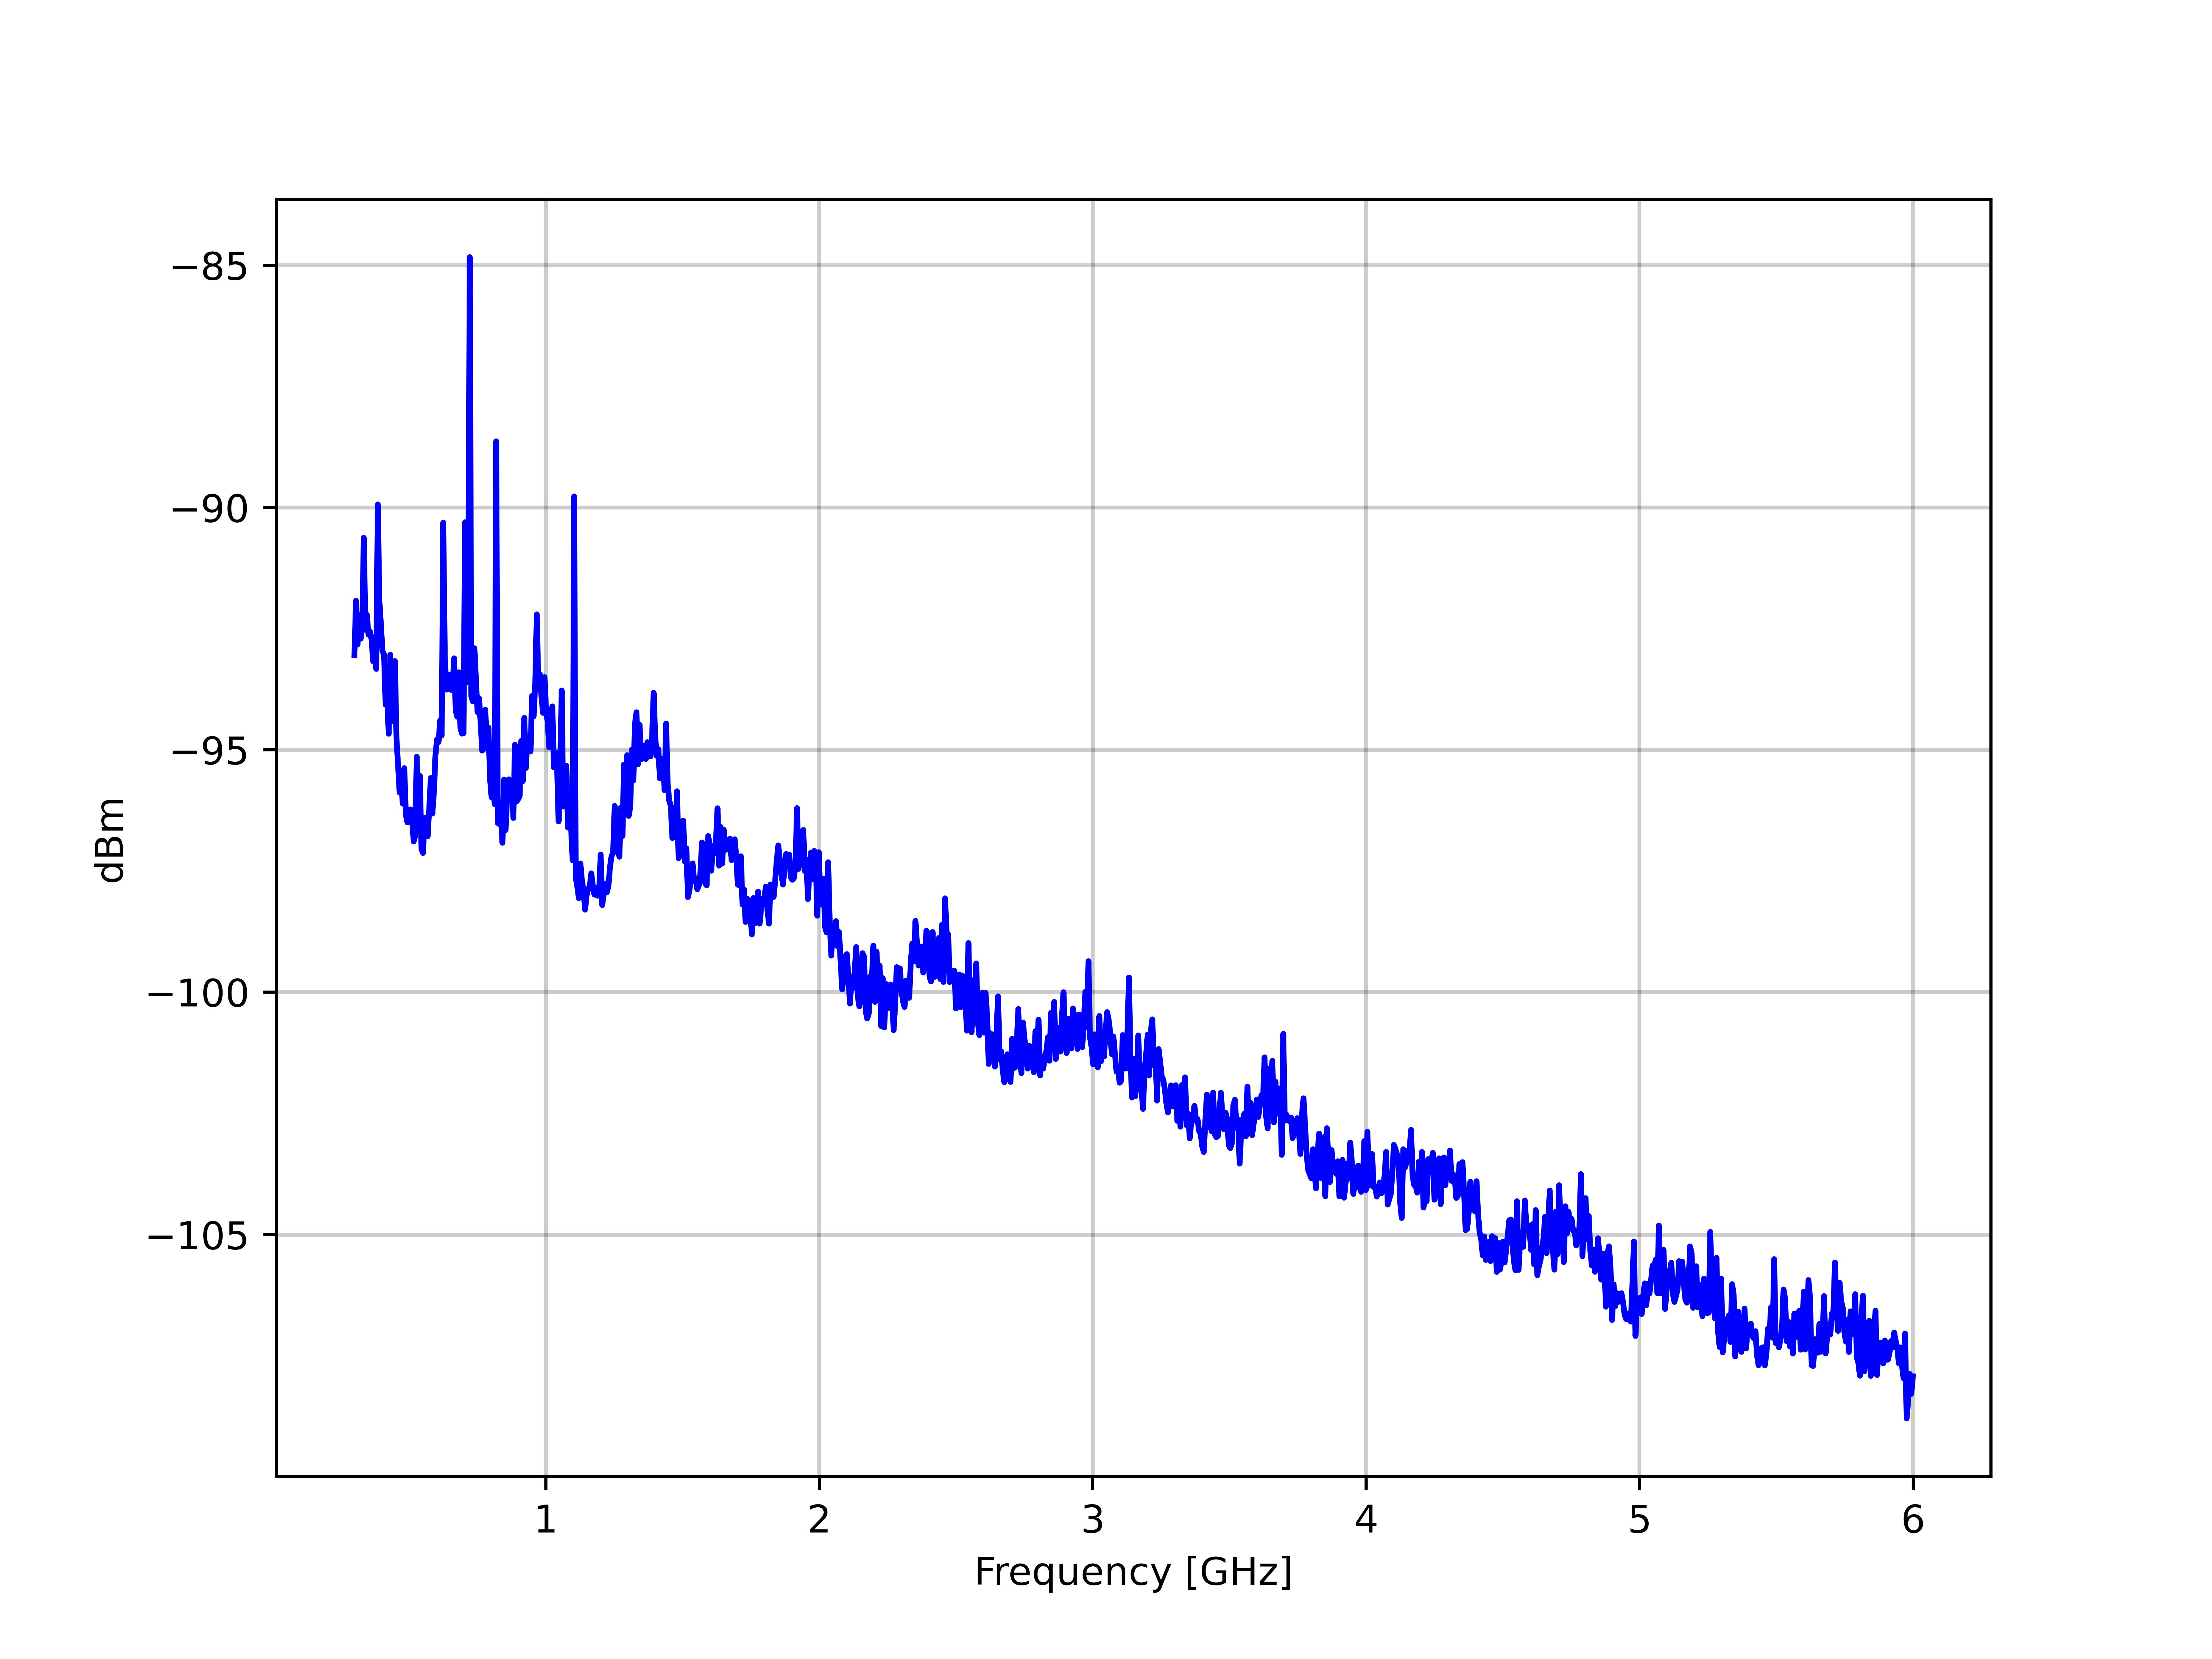
\includegraphics[width=0.9\linewidth]{Figures/baseline_spectrum.jpg}
\caption{Baseline spectrum for the GReX EMI measurements.}
\label{fig:baseline_result}
\end{figure}
%
\begin{figure}[H]
\centering
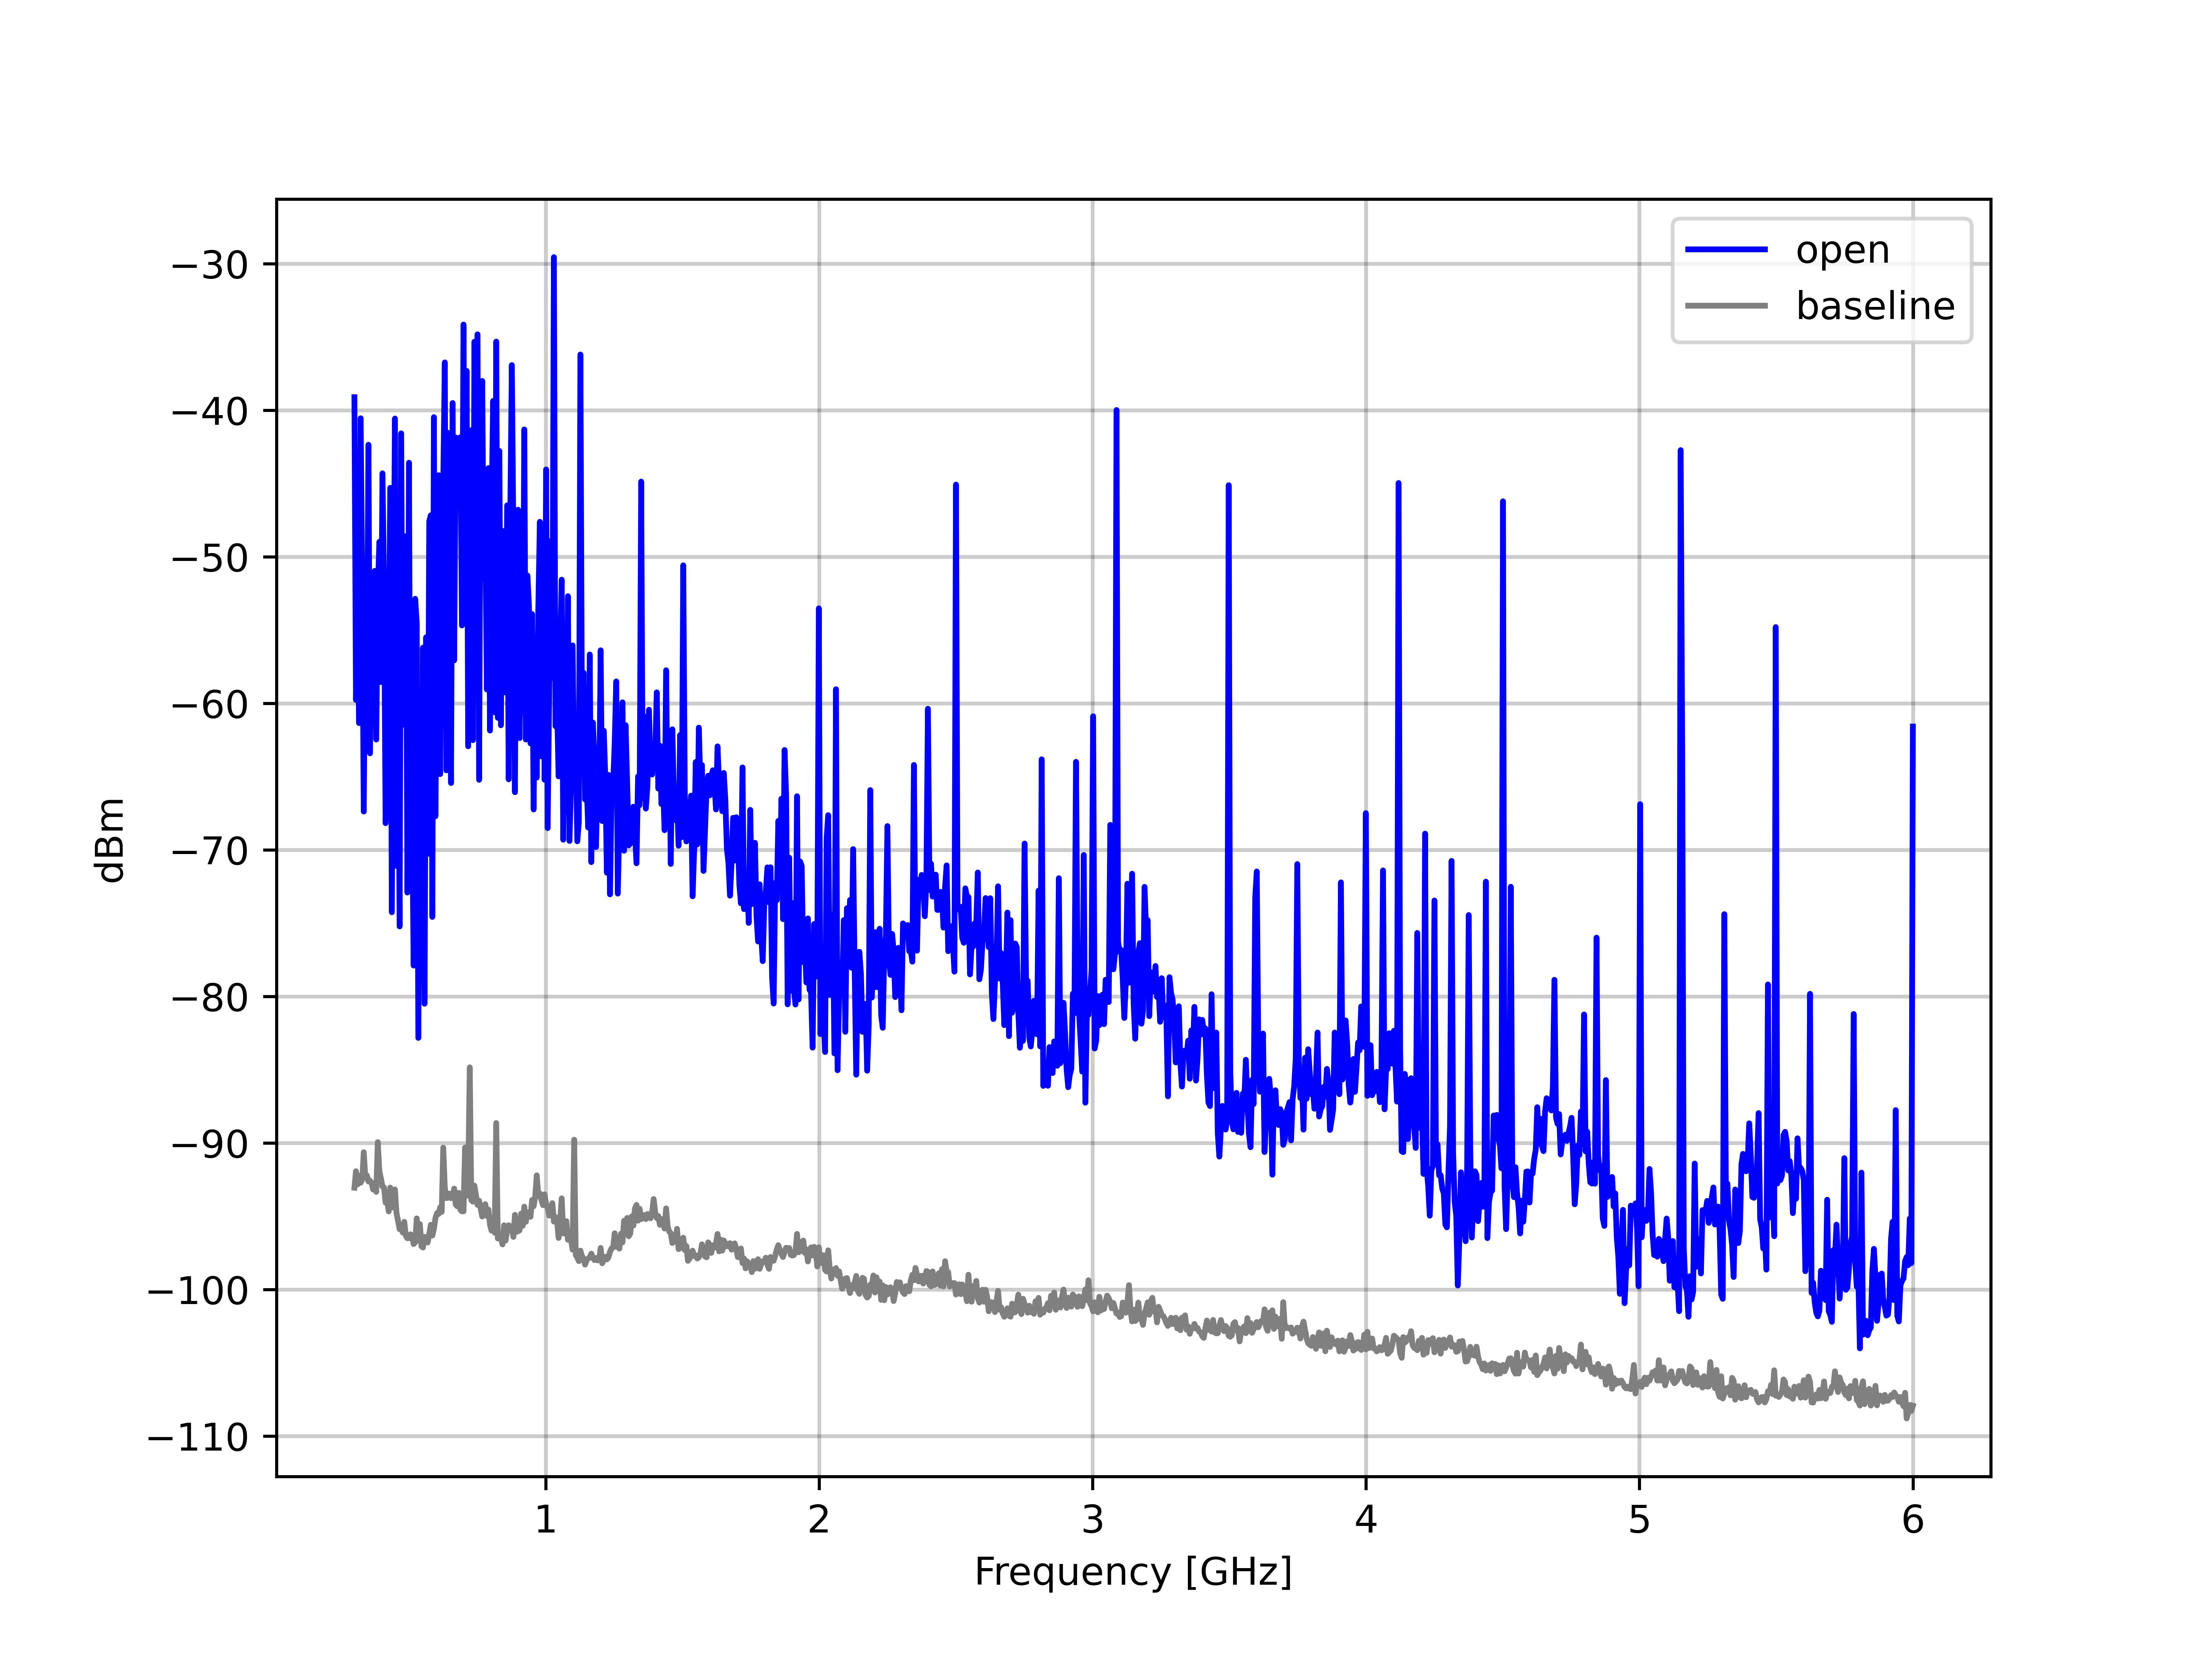
\includegraphics[width=0.9\linewidth]{Figures/open_comparison_spectrum.jpg}
\caption{EMI emission spectrum of the GReX unit with its enclosure opened, compared with the baseline spectrum.}
\label{fig:open_result}
\end{figure}
%
\begin{figure}[H]
\centering
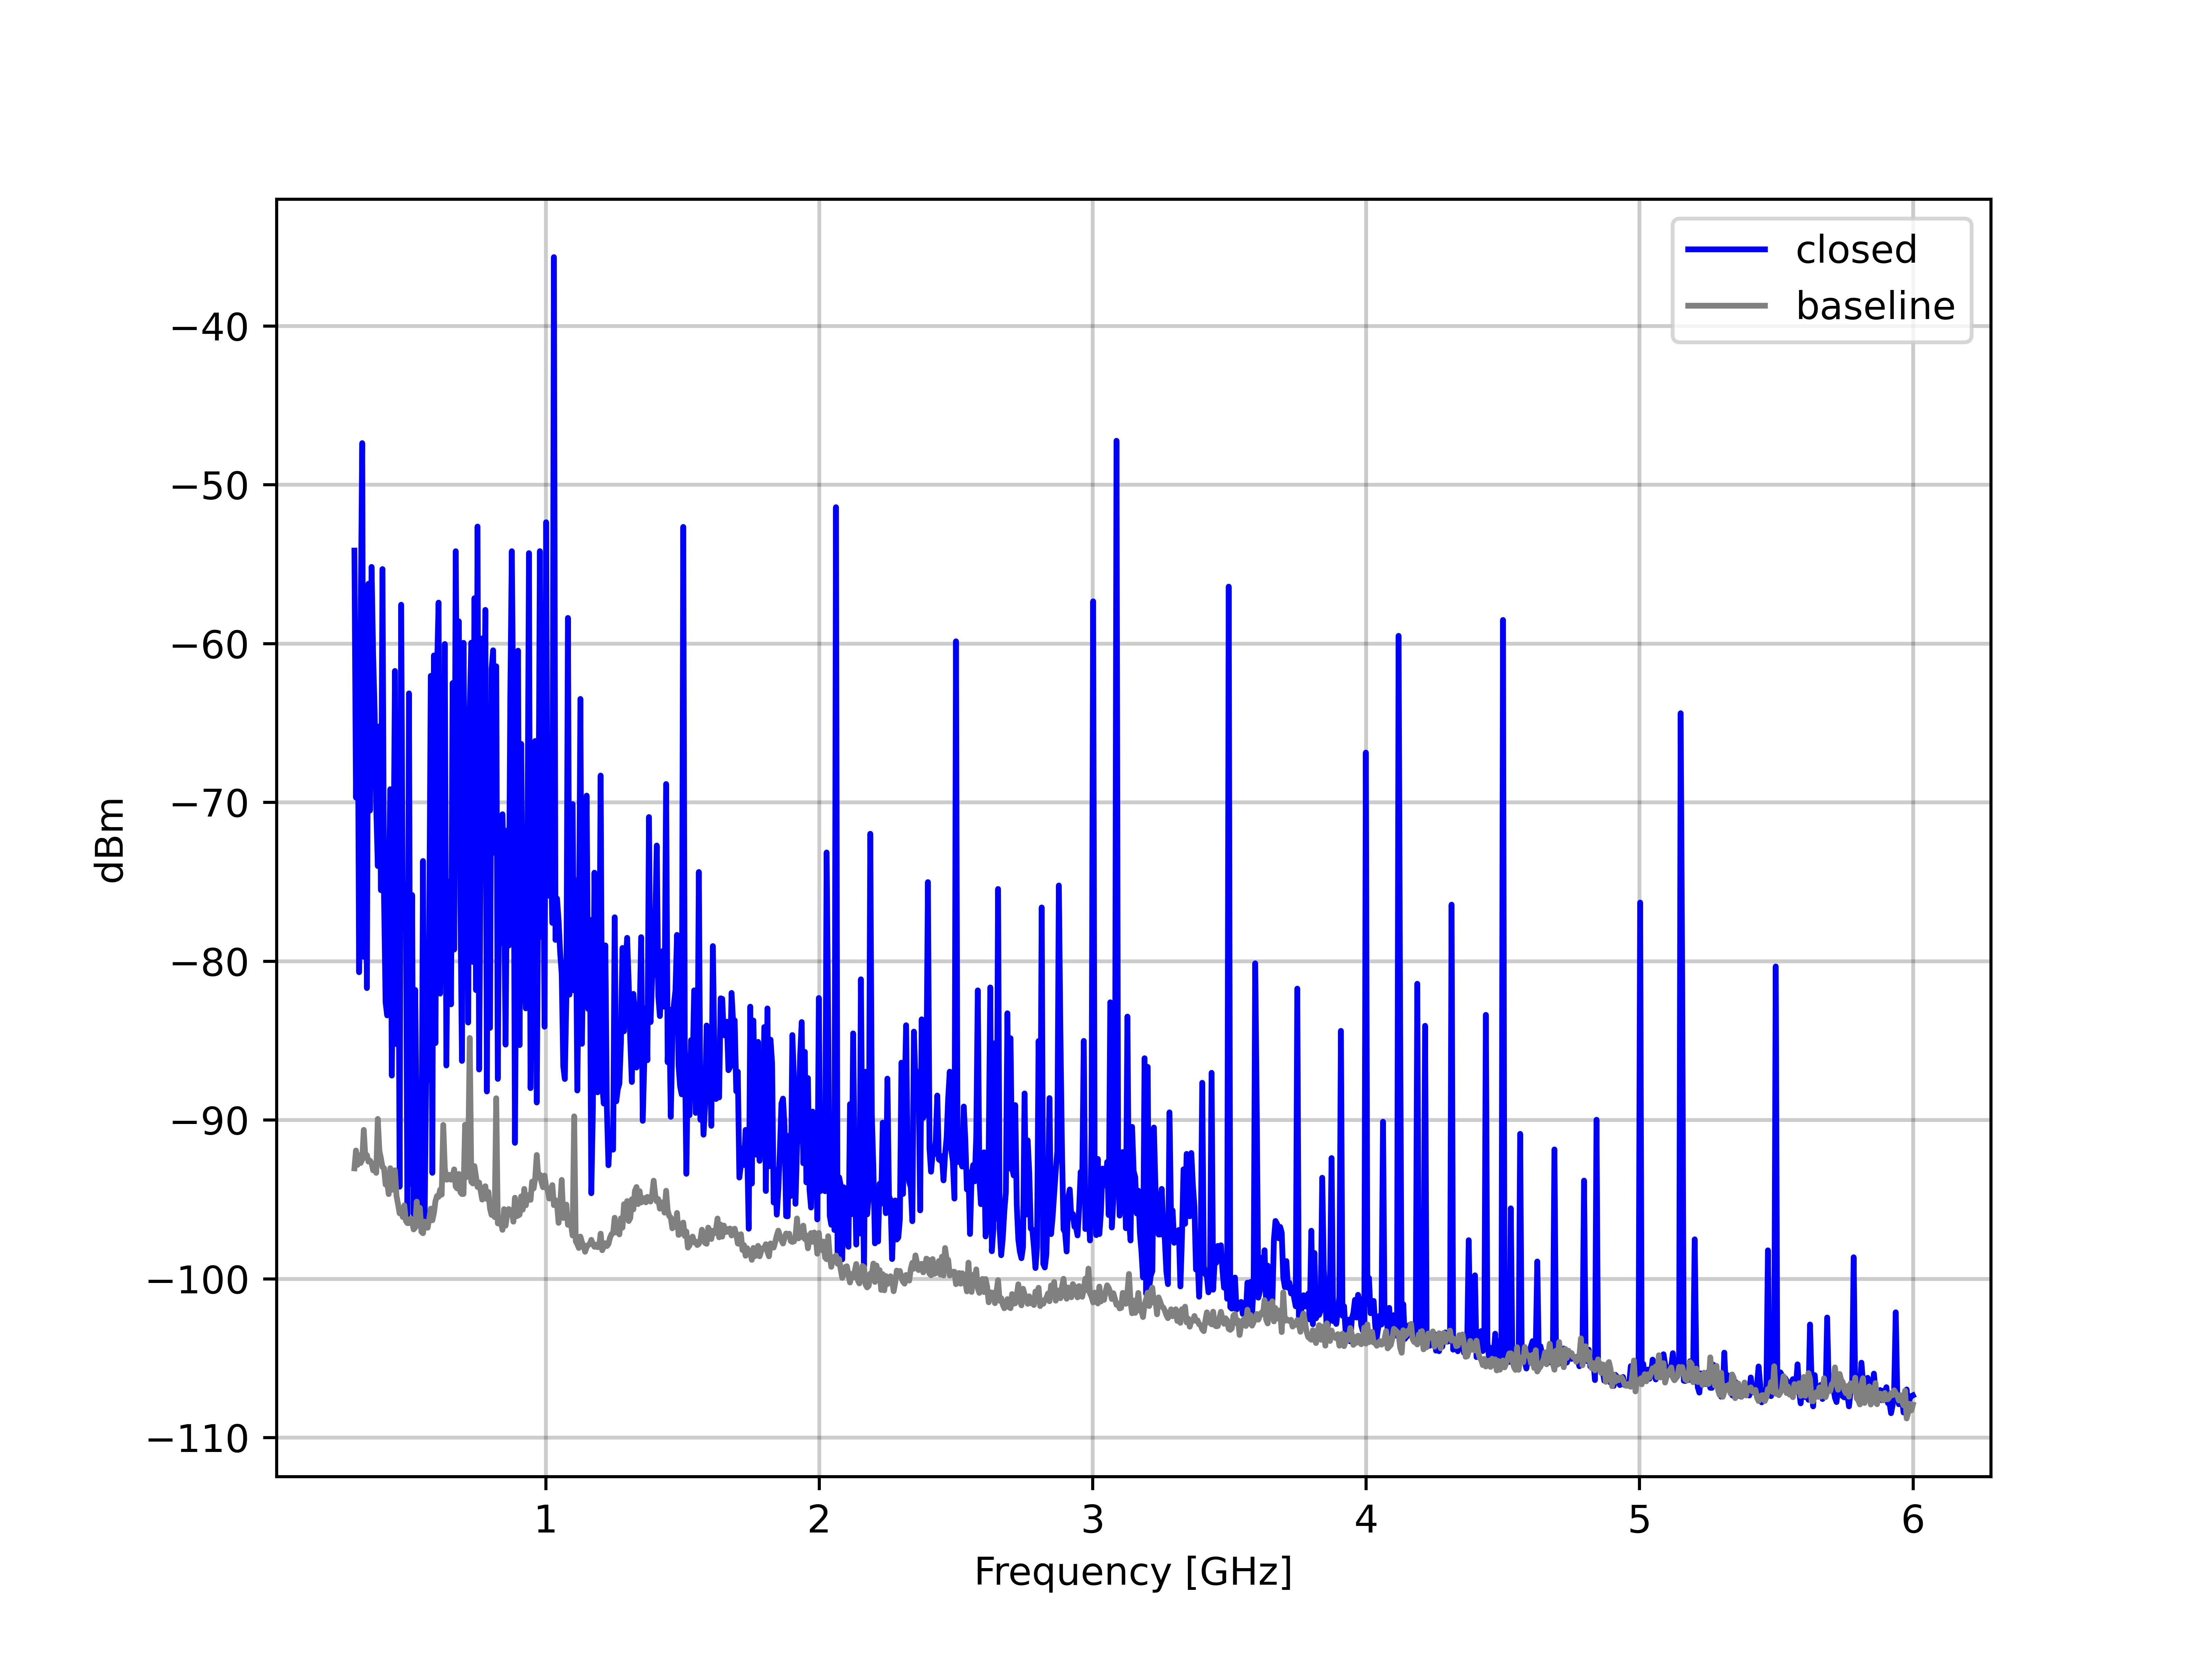
\includegraphics[width=0.9\linewidth]{Figures/closed_comparison_spectrum.jpg}
\caption{EMI emission spectrum of the GReX unit with its enclosure closed, compared with the baseline spectrum.}
\label{fig:closed_result}
\end{figure}
%
\begin{figure}[H]
\centering
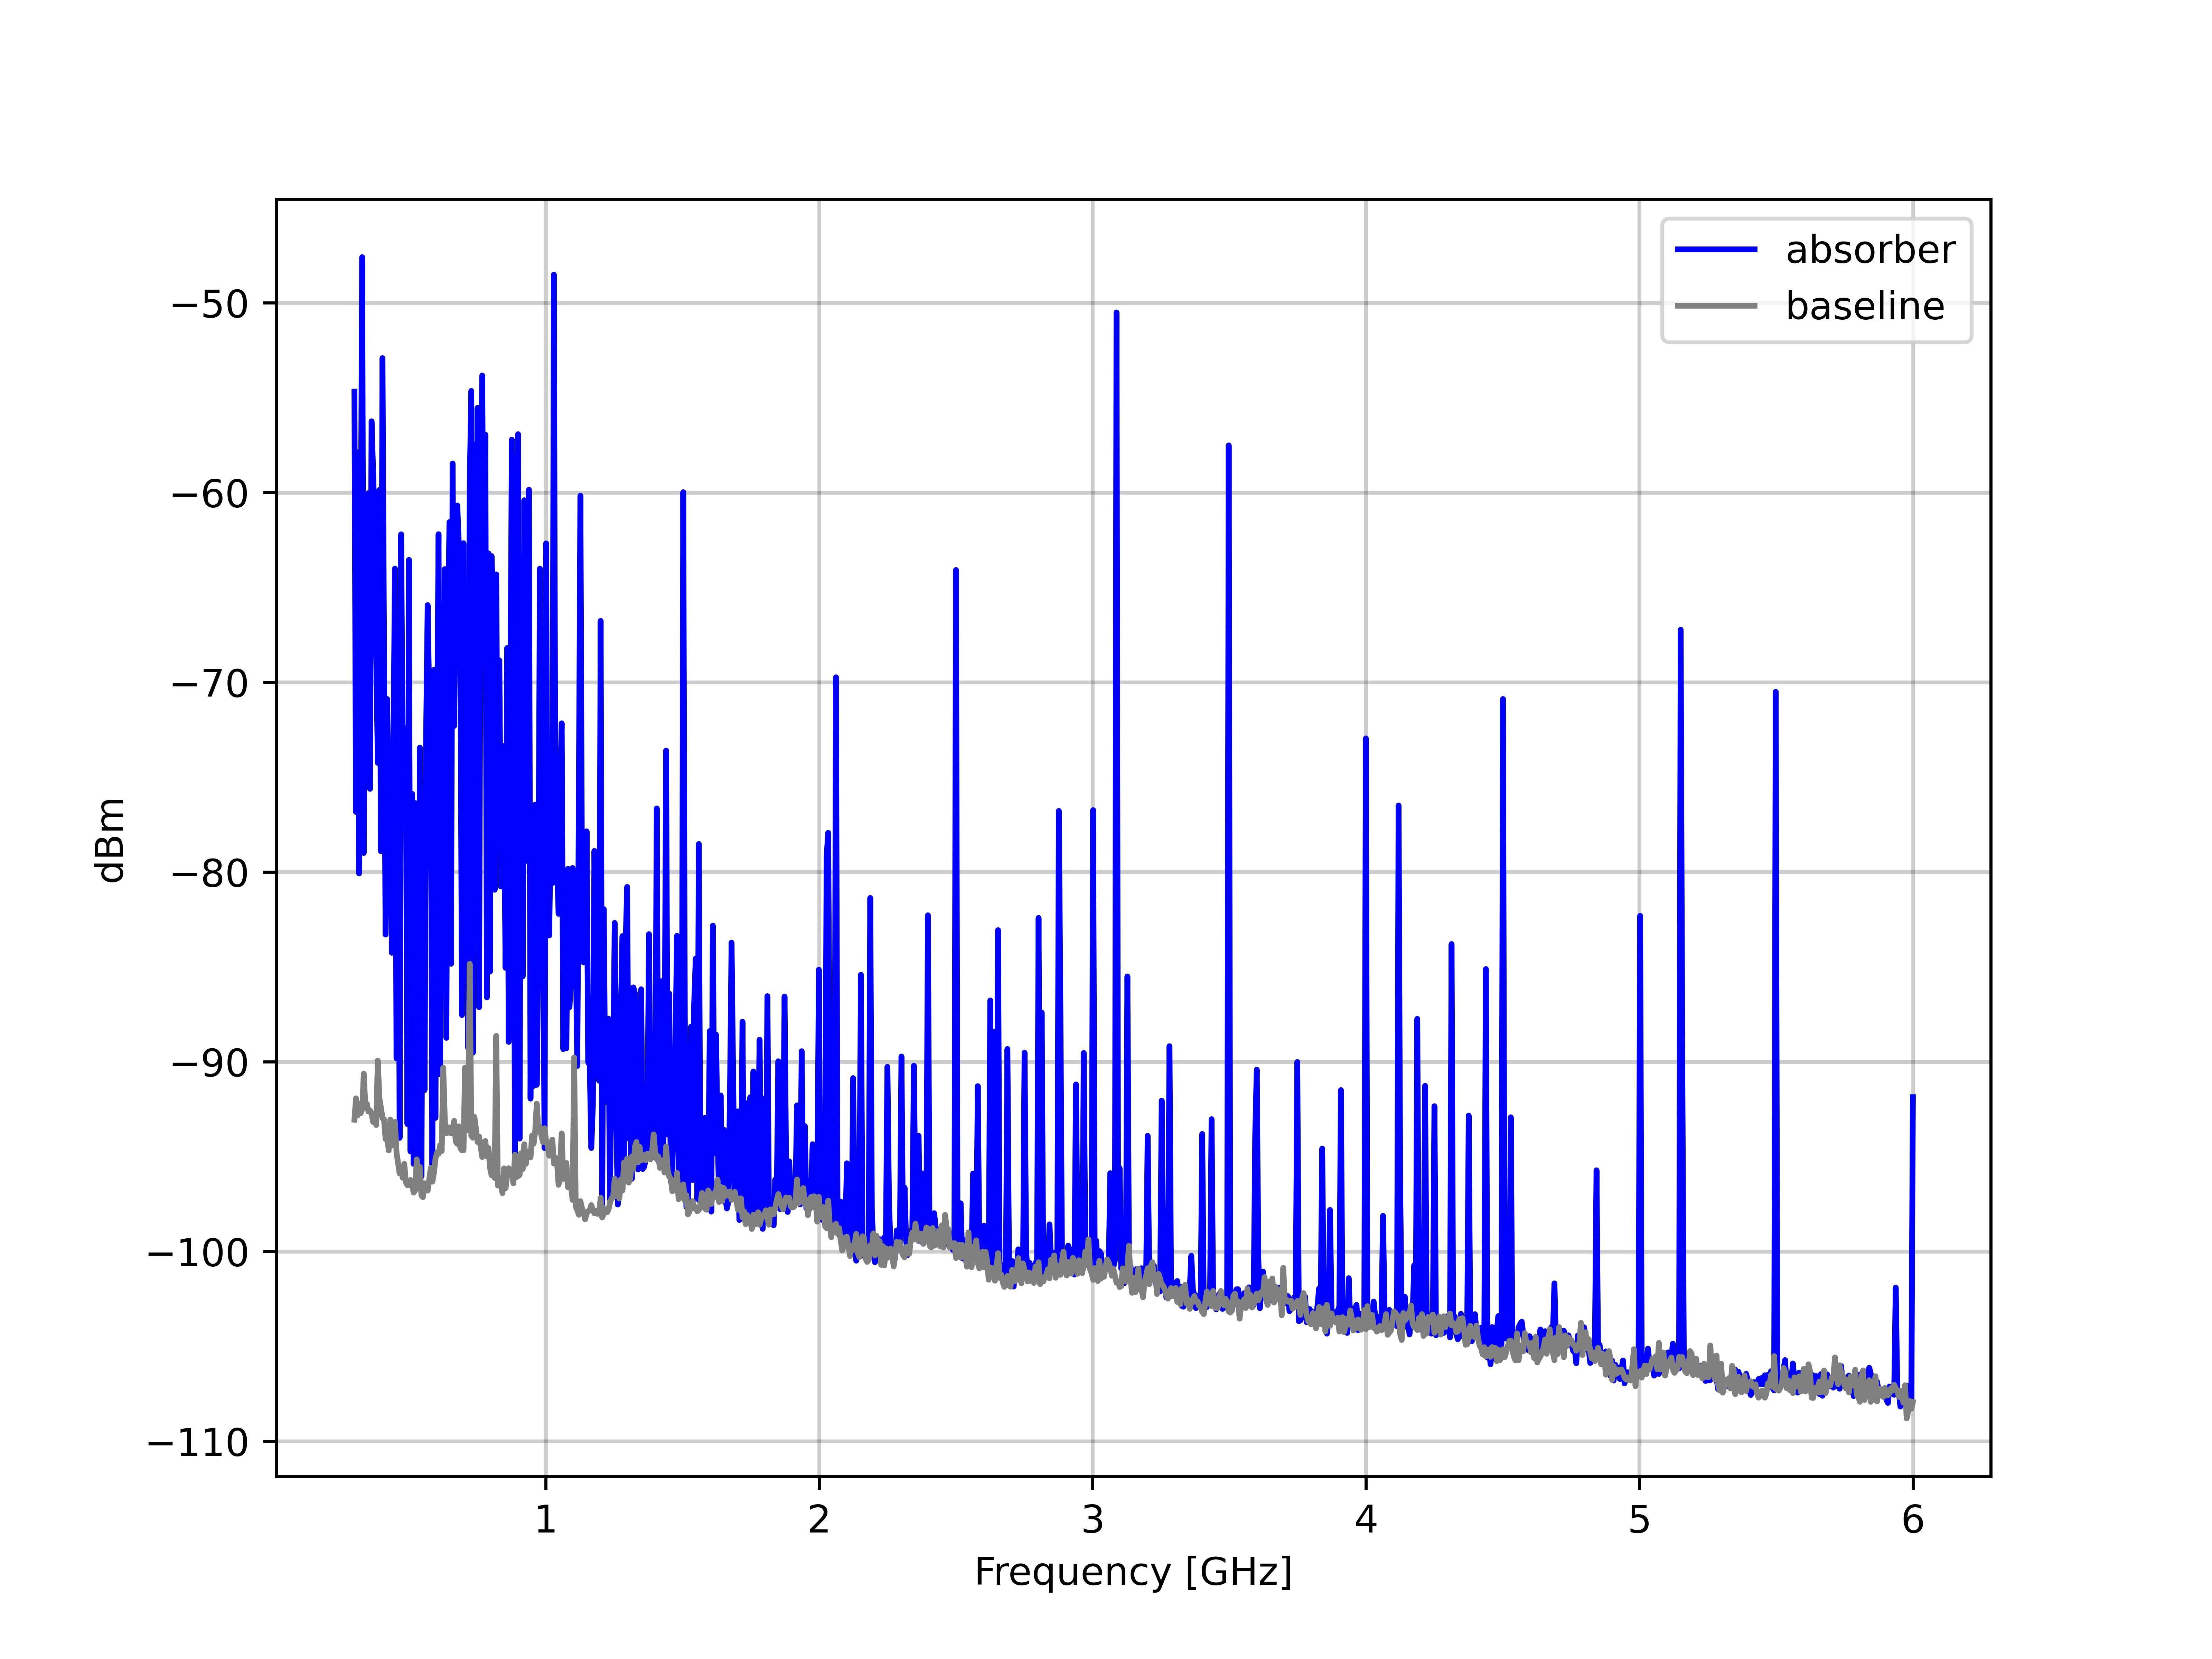
\includegraphics[width=0.9\linewidth]{Figures/absorber_comparison_spectrum.jpg}
\caption{EMI emission spectrum of the GReX unit with its enclosure closed and absorbers added inside the enclosure, compared with the baseline spectrum.}
\label{fig:absorber_comparison_spectrum}
\end{figure}


\begin{table}[]
    \centering
   
    \begin{tabular}{|c|c|c|}
    \hline
         \cellcolor[gray]{0.85} Measurement & \cellcolor[gray]{0.85} Frequency [GHz] &  \cellcolor[gray]{0.85} Amplitude [dBm]\\ \hline
         open & 3.0873 & -39.978501 \\ \hline
         open & 3.4977 & -45.107806 \\ \hline
         open & 4.1190 & -44.959350 \\ \hline
         open & 4.5009 & -46.206643 \\ \hline
         open & 5.4984 & -54.792139 \\ \hline
         \hline
         closed & 0.4995 & -63.143009 \\ \hline
         closed & 1.0296 & -35.672183 \\ \hline
         closed & 1.5027 & -52.661033 \\ \hline
         closed & 2.0613 & -51.418850 \\ \hline
         closed & 2.5002 & -59.862832 \\ \hline
         closed & 3.0018 & -57.345924 \\ \hline
         closed & 3.0873 & -47.234282 \\ \hline
         closed & 3.4977 & -56.419926 \\ \hline
         closed & 3.9993 & -66.870435 \\ \hline
         closed & 4.5009 & -58.519204 \\ \hline
         \hline
         absorber & 1.0296 & -48.517166 \\ \hline
         absorber & 2.5002 & -64.079893 \\ \hline
         absorber & 3.0873 & -50.503989 \\ \hline
         absorber & 3.4977 & -57.511396 \\ \hline
         absorber & 3.9993 & -72.956611 \\ \hline
         absorber & 4.5009 & -70.879781 \\ \hline
         absorber & 5.4984 & -70.499525 \\ \hline

    \end{tabular}
    \caption{List of main emission peaks in the spectrum recorded for the GReX EMI measurements. Computed using scipy.signal's find\_peaks function (threshold: 30, distance: 5).}
    \label{tab:main_emission_peaks}
\end{table}


\end{document}

